\documentclass[a4paper]{article}
\usepackage{hyperref}
\usepackage{graphicx}
\usepackage{caption}
\usepackage{subcaption}
\usepackage{listings}
\graphicspath{ {./images/} }

\title{SON implementation on Spark in python}
\author{Carli Alberto VR473845\and Fraccaroli Leonardo VR??????}
\date{}

\begin{document}
	\maketitle
	\tableofcontents
	\medskip
	\section{Introduction}
	Finding frequent itemsets is frequently done in data mining domains to understand which items frequently appear together. The definition of "items" is beyond the scope of this work. Suffice to say that we treated them as binary variables, listed in a basket only when their value is True. In out project a basket is a list of items that appear together.\\
	
	This is an analysis that can be performed on almost any dataset, but is especially suited for domains like e-commerce. It is an interesting challenge to try and take the system to the extreme where the dataset is so large that it does not fit on any single machine's memory and it is more convenient to distribute analysis to multiple compute units.\\
	
	We tried to imagine ourselves into a big e-commerce company that stores transaction data on a distributed database and wants to periodically analyse data to understand which items are usually bought together. \\
	The data is simply a list of items bought at any one time; as the distributed database we used MongoDB and thus we needed a version of parallel apriori. \\
	We tried to parallelize apriori by using Spark on python and using the SON algorithm as proposed in chapter 6.4.4 of the \href{http://www.mmds.org/}{Mining Massive Datasets} book.
	\newpage

	\section{SON}
	In this section we will dissect our implementation of SON through Spark on python, describing all the steps of computation and their result.\\
	
	\subsection{SON Algorithm}	
	The algorithm as described in the book involves two phases of mapreduce as follows:
	\begin{enumerate}
	\item The map basically executes apriori on a batch of baskets, extracting all frequent itemsets. The required frequency (support) is reduced by a factor equal to the number of number of batches the data is partitioned in.\\
	The reducer is an identity reducer and simply combine all the frequent itemsets from every basket in a single list. These are candidate frequent itemsets.
	\item The map function takes a batch of the data and counts every occurrence of every itemset in the candidates list. The reducer adds up the counts from every batch and finally filters out the infrequent ones using the original support.
	\end{enumerate}
	The result of this is the list of frequent itemsets without false positives.
	
	\subsection{Our Implementation}
	Our implementation expects a $pyspark$ RDD\\
	
	\subsubsection{First Map}
	The input data is in the form of a list of lists, where every internal list holds a set of strings, which are the items (fig: \ref{fig:input_data}).\\
	
	Apriori algorithm is applied to every batch, which returns a list of frequent itemsets (fig: \ref{fig:apriori}). This is done with the $mapPartitions$ function of $pyspark$: 
	\begin{lstlisting}[language=Python]
.mapPartitions(lambda x: apriori(list(x), chunk_support))
	\end{lstlisting}	
	We will discuss our implementation of apriori, in details, in section \ref{section:apriori}. We chose not to keep only the largest set because we saw that there may be cases where the larger set is not globally supported, but the smaller ones are.\\
	Then every itemset is "emitted" with a 1, to facilitate the reduce phase:
	\begin{lstlisting}[language=Python]
.map(lambda x: (x, 1))
	\end{lstlisting}
	
	\subsubsection{First Reduce}
	Now the result of the previous step is grouped by key (fig: \ref{fig:grouped}) and the list of counts discarded entirely:
	\begin{lstlisting}[language=Python]
.groupByKey()
.map(lambda x: x[0])
	\end{lstlisting}
	The result is the list of all itemsets that appear at least once (fig: \ref{fig:candidate_fi}), which means that they are frequent in at least one batch.
	
	\begin{figure}[h]
		\centering
		
		\begin{subfigure}[b]{0.24\textwidth}
			\centering
			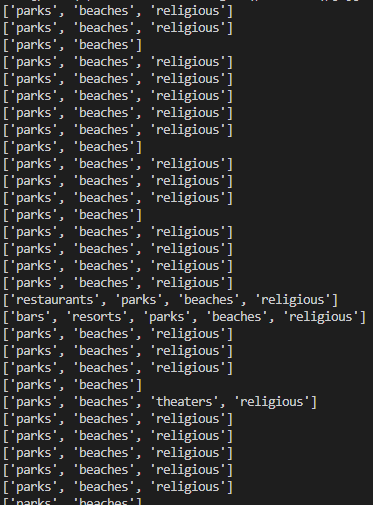
\includegraphics[width=\textwidth]{Baskets.PNG}
         	\caption{Input data}
         	\label{fig:input_data}
		\end{subfigure}
		\hfill
		\begin{subfigure}[b]{0.24\textwidth}
			\centering
			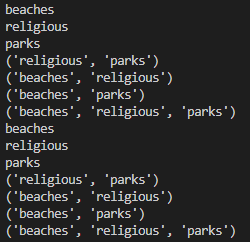
\includegraphics[width=\textwidth]{Batch_fi.PNG}
         	\caption{Apriori on batch}
         	\label{fig:apriori}
		\end{subfigure}
		\hfill
		\begin{subfigure}[b]{0.24\textwidth}
			\centering
			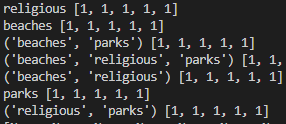
\includegraphics[width=\textwidth]{grouped.PNG}
         	\caption{First reduce}
         	\label{fig:grouped}
		\end{subfigure}
		\hfill
		\begin{subfigure}[b]{0.24\textwidth}
			\centering
			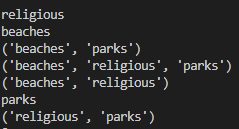
\includegraphics[width=\textwidth]{candidates.PNG}
         	\caption{Candidate frequent itemsets}
         	\label{fig:candidate_fi}
		\end{subfigure}
	
	\end{figure}
	
	\subsubsection{Second Map}
	At this point our candidate frequent itemsets are still partitioned. We need to distribute the whole list to every batch of data. In order to do so we coalesced the candidates RDD into one single partition, group it together and multiply if with every partition of the original data:
	\begin{lstlisting}[language=Python]
.repartition(1)
.glom()
.cartesian(baskets.glom())
	\end{lstlisting}
	The result is, for every partition, a list containing two lists; the first one is a list of itemsets and the second one is the batch of data (fig: \ref{fig:cartesian}).\\
	Then, for every itemset in the first list, we count in how many baskets is present\footnote{count\_frequencies is a function we developed that does exactly that: count the occurrences of the elements in the first list in the second list}:
	\begin{lstlisting}[language=Python]
.mapPartitions(lambda x : count_frequencies(list(x)[0])) 
	\end{lstlisting}
	The result is a list of tuples where the first element is the itemset and the second is the count for every batch (fig: \ref{fig:counts}).
	
	
	\subsubsection{Second Reduce}
	Now the itemsets are reduced across partitions by summing counts (fig: \ref{fig:totals}) and then filtered:
	\begin{lstlisting}[language=Python]
.reduceByKey(lambda x, y: x + y)
.filter(lambda x: x[1] / data_size >= support)
	\end{lstlisting}
	
	The result is the list of every itemset which is supported enough to be considered frequent. Our next step is to filter out all the smaller sets which are included in larger sets.
	
	
		
	\begin{figure}[h]
		\centering
		
		\begin{subfigure}[b]{0.3\textwidth}
			\centering
			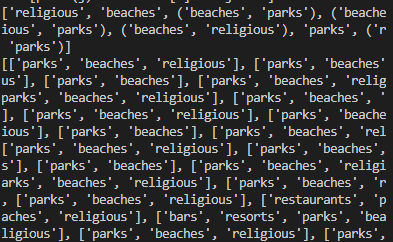
\includegraphics[width=\textwidth]{cartesian.PNG}
         	\caption{Cartesian product result}
         	\label{fig:cartesian}
		\end{subfigure}
		\hfill
		\begin{subfigure}[b]{0.3\textwidth}
			\centering
			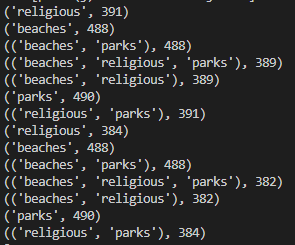
\includegraphics[width=\textwidth]{counts.PNG}
         	\caption{Counts of itemsets for every batch}
         	\label{fig:counts}
		\end{subfigure}
		\hfill
		\begin{subfigure}[b]{0.3\textwidth}
			\centering
			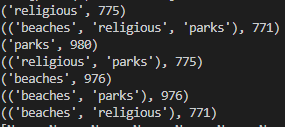
\includegraphics[width=\textwidth]{totals.PNG}
         	\caption{Sum of counts across partitions}
         	\label{fig:totals}
		\end{subfigure}
	\end{figure}
	
	\newpage
	
	\section{apriori}
	\label{section:apriori}
	
	Apriori is the most used algorithm to find frequent itemsets in a dataset. The algorithm relies on the monotonicity of support by building candidates from smaller sets which are knowingly frequent. This is because it is impossible for an itemset to be frequent if every item it is composed of is frequent by itself.\\
	
	To benchmark SON execution we had to compare it to an implementation of apriori, which we made ourselves:
	\begin{lstlisting}[language=Python]
def apriori(data, support):
    basket_size = len(data)
    frequent_itemsets = []
    items = list(set([k for j in data for k in j]))
    temp = count_frequencies((items, data))
    frequent_items = [i[0] for i in temp if i[1]/basket_size >= support]
    new_frequent_itemsets = frequent_items
    while new_frequent_itemsets != []:
        frequent_itemsets += new_frequent_itemsets
        new_candidate_itemsets = [(j, ) + (k, ) if isinstance(j, str) \
        	else j + (k,) for j in new_frequent_itemsets \for
        	k in frequent_items if k not in j]
        new_candidate_itemsets = [tuple(j) for j in {frozenset(i) \
        for i in new_candidate_itemsets}]
        temp = count_frequencies((new_candidate_itemsets, data))
        new_frequent_itemsets = [i[0] for i in temp \
        if i[1]/basket_size >= support]
    return frequent_itemsets	
    \end{lstlisting}
    This code first extracts the items from the data, keeps the frequent ones and then uses them to build all the candidate couples, counts them, filters out infrequent ones and then expands those couples to form triples and so on.
	
	\section{benchmark}
	We have ran some benchmarks to better understand how SON compares to apriori.\\
	In order to do so we made a script for the specific purpose of being able to programatically change parameters and 
	subsample datasets.
	Also, we implemented a gridsearch to test many parameters. We also added a logging feature to our project to better follow executions and ease debug.
	We compared our implementation, both based on DB and in memory, to a method $FreqItems$ provided by $pyspark.sql$. 
	This function uses a modified version of FP-Tree to be more parallelizeable. This function proved itself to be absurdly fast, at the expense of false positives.
	Both a  `simple' dataset and a `harder' one were used to compare performances.

	\subsection{Datasets}
	The first "easier" dataset is from UCI \href{https://archive.ics.uci.edu/ml/datasets/Travel+Reviews#}{(Travel Reviews)} and is composed of averages of scores that every user gave to some
	categories of places on TripAdvisor. We rounded the scores to integer and kept only the ones above 3.\\
	This way our dataset is in the form:\\
	user\_id: category1, category2 \ldots\\
	It is considered "easy" because it is very sparse and the number of items is very low.\\

	The second "harder" dataset is a collection of transaction where some user bought some item in a transaction, again from UCI \href{https://archive.ics.uci.edu/ml/datasets/online+retail}{(Online Retail)}.
	We decided to form transactions on invoices, so we extracted the list of items bought together.
	This way our dataset is in the form:\\
	invoice\_no: item\_code, item\_code \ldots\\
	It is considered "harder" because of the higher number of items.\\

	\subsection{Results}
	% Setups (CPU, MEMORY, MONGO)
	These tests were performed on an 8 core $i5-8250U @1.6GHz$, with 16 GB DDR4 memory $@2400MHz$, but both the driver and the executor were capped at 4 GB.
	figures \ref{fig:easybenchmark}, \ref{fig:hardbenchmark}

	\begin{figure}[h]
		\centering
		\begin{subfigure}[b]{1\textwidth}
			\centering
			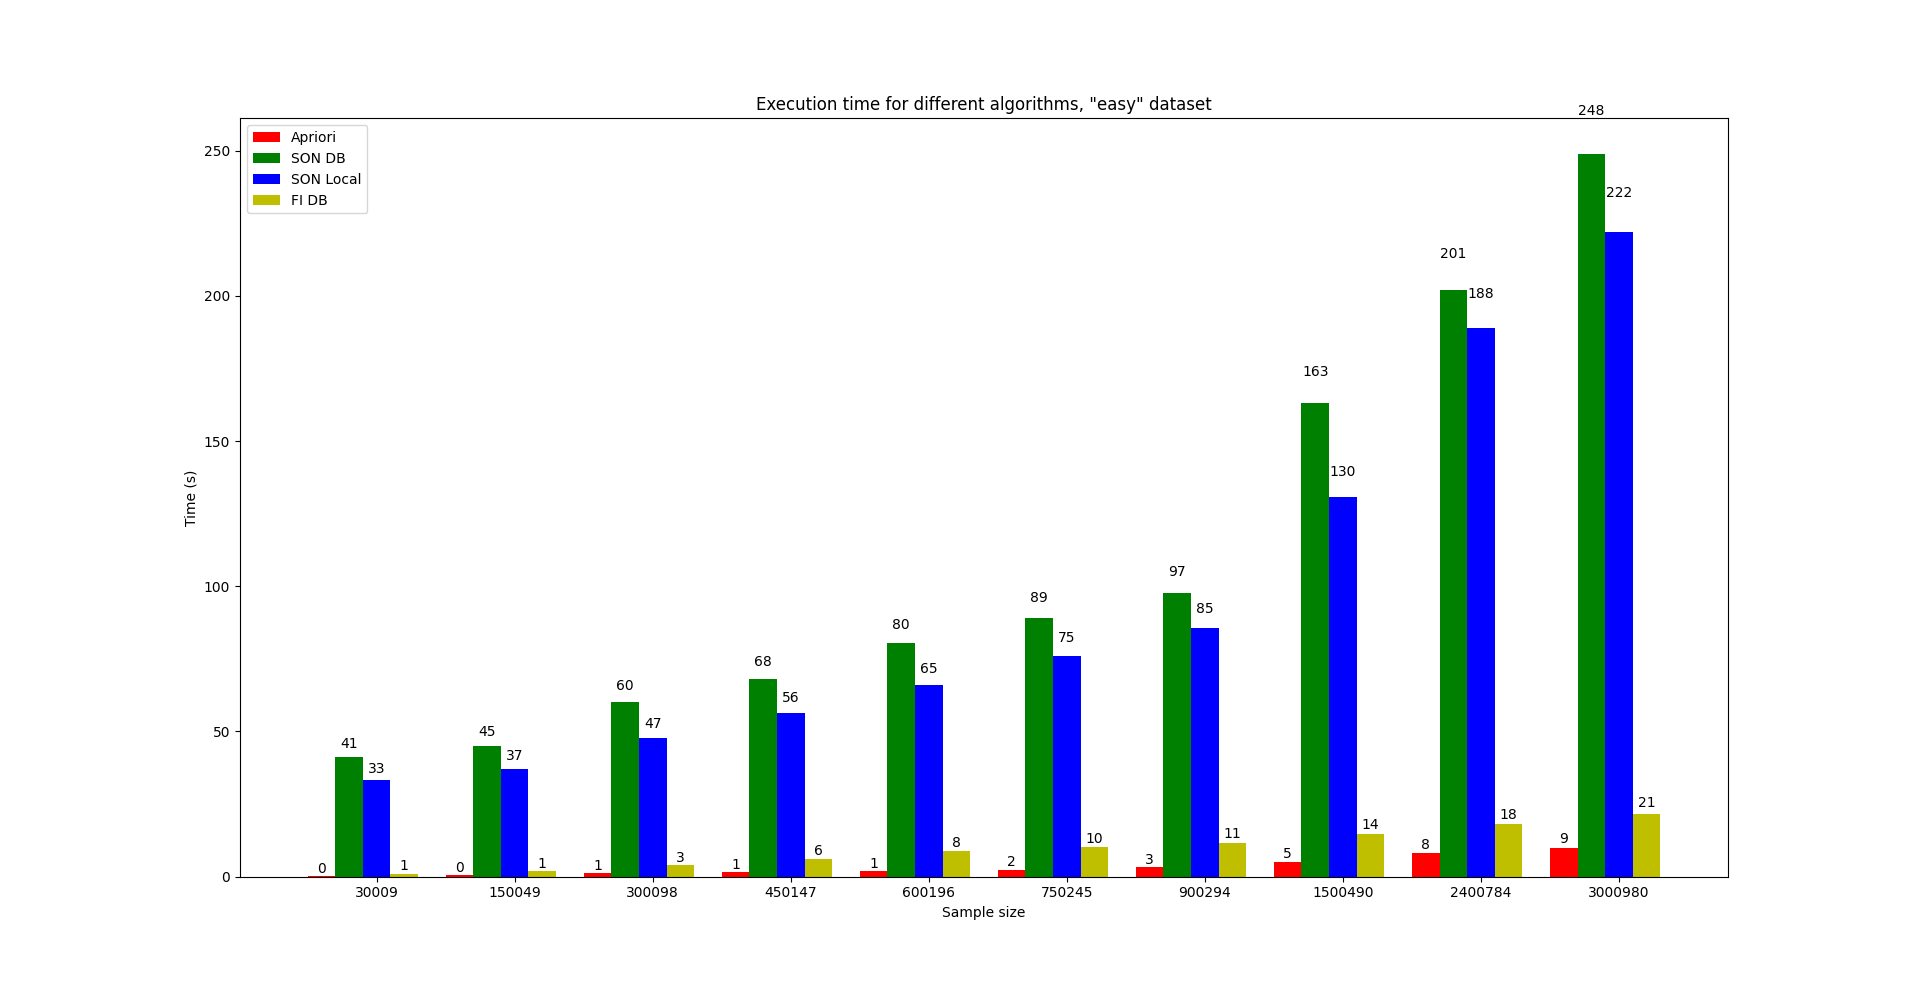
\includegraphics[width=\textwidth]{benchmarkeasy.png}
         	\caption{Easy dataset benchmark results}
         	\label{fig:easybenchmark}
		\end{subfigure}
		\hfill
		
		\begin{subfigure}[b]{1\textwidth}
			\centering
			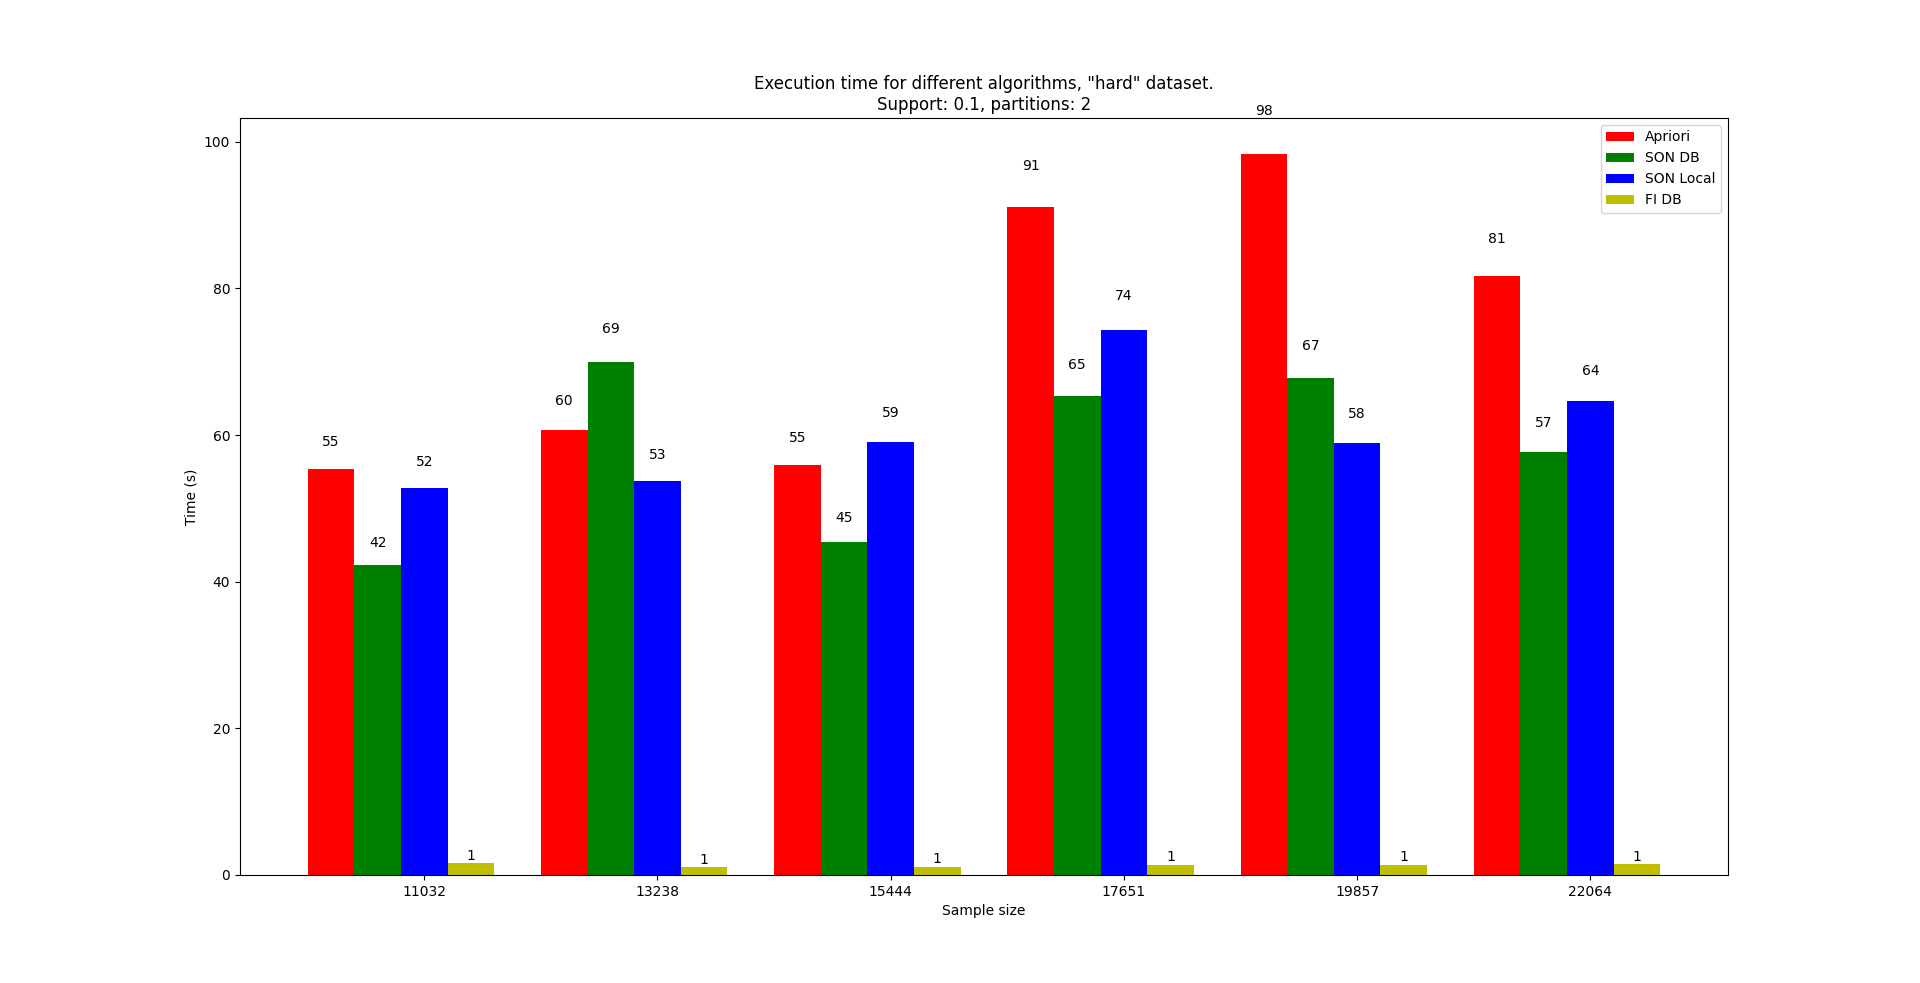
\includegraphics[width=\textwidth]{benchmarkhard.png}
         	\caption{Hard dataset benchmark results}
         	\label{fig:hardbenchmark}
		\end{subfigure}
		\hfill
		
	\end{figure}

	
	\section{Conclusions}
	The main advantage of SON, that we could appreciate in our single machine setup, was the ability to use all available core, distributing the load.\\
	But aside from that, we appreciated how the algorithm is slow and only to be used when needed. It is not to be preferred to apriori or FP-Trees.\\
	We have seen how easy it is connecting pyspark to a distributed database, eventually sharded.\\

	With the testing we have appreciated how SON execution time remains somewhat constant, while apriori execution time grows exponentially with the number of items.\\
	Also, because of the way SON works, we expect to work better on denser datasets and with a higher number of items, because the splitting of the datasets produces
	smaller exponentiation in the number of candidates.\\
	
	After the benchmarks it is clear that apriori is blazingly fast and the only reasons one should instead use SON is when data doesen't fit in memory or many compute units are available.
	
\end{document}